\begin{figure}[t]
\centering
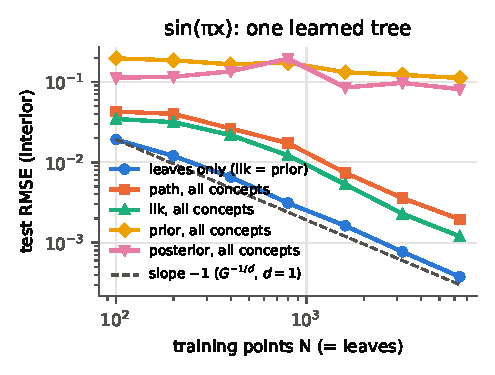
\includegraphics[width=0.48\linewidth]{figs/weighting_sin.pdf}\hfill
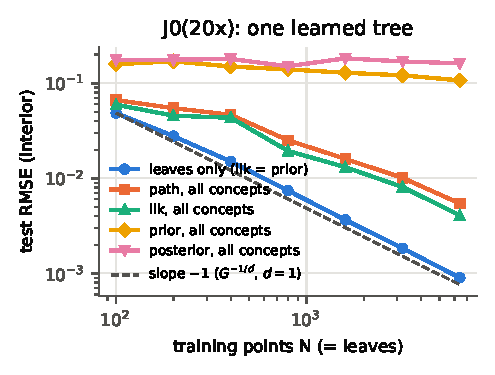
\includegraphics[width=0.48\linewidth]{figs/weighting_j0.pdf}
\caption{One learned tree, variance floor at the data spacing, full expansion.  The
leaves-only mixture falls with slope $-1$; the \textsc{path} and \textsc{lik} mixtures
over all concepts fall more slowly; the \textsc{prior} mixture over all concepts falls only
like $1/\log N$ and the \textsc{posterior} mixture stays high (\cref{rem:hierarchy}).
Numbers in \cref{tab:weighting}.}
\label{fig:weighting}
\end{figure}

\begin{table}[t]
\centering\small
\begin{tabular}{@{}llrrrr@{}}\toprule
target & mixture & $N=100$ & $N=400$ & $N=1600$ & $N=6400$\\\midrule
$\sin(\pi x)$ & leaves only & 0.019 & 0.0066 & 0.0016 & 0.00038\\
$\sin(\pi x)$ & path, all & 0.043 & 0.026 & 0.0074 & 0.002\\
$\sin(\pi x)$ & lik, all & 0.035 & 0.022 & 0.0053 & 0.0012\\
$\sin(\pi x)$ & prior, all & 0.197 & 0.166 & 0.132 & 0.112\\
$\sin(\pi x)$ & posterior, all & 0.113 & 0.135 & 0.085 & 0.081\\
$J_0(20x)$ & leaves only & 0.049 & 0.015 & 0.0037 & 0.0009\\
$J_0(20x)$ & path, all & 0.066 & 0.047 & 0.016 & 0.0054\\
$J_0(20x)$ & lik, all & 0.059 & 0.043 & 0.013 & 0.0041\\
$J_0(20x)$ & prior, all & 0.158 & 0.150 & 0.129 & 0.107\\
$J_0(20x)$ & posterior, all & 0.175 & 0.180 & 0.183 & 0.162\\
\bottomrule\end{tabular}
\caption{Interior test RMSE of one learned tree (mean of three seeds), the data of
\cref{fig:weighting}.}
\label{tab:weighting}
\end{table}

\Cref{fig:weighting,tab:weighting} show the four weightings on learned trees.  These runs
are outside the hypotheses of \cref{thm:single,prop:prior}, which concern a constructed
grid tree, and of \cref{thm:consistency}: the variance floor equals the data spacing
($h\asymp1/N$), the interpolation regime of a noise-free target, not the regime
$Nh^d\to\infty$.  They show the same pattern as the constructions: for $\sin(\pi x)$ the
leaves-only error falls from $0.019$ at $N=100$ to $0.00038$ at $N=6400$, a factor of about
four per quadrupling of $N$, while the \textsc{prior} mixture over all concepts stays
between $0.11$ and $0.20$ and the \textsc{posterior} mixture between $0.08$ and $0.14$ at the tabulated $N$ (and
$0.19$ at $N=800$ in the figure)
(between $0.15$ and $0.19$ for $J_0(20x)$).

\begin{table}[t]
\centering\small
\resizebox{\linewidth}{!}{\begin{tabular}{@{}rrrrrrrrrrr@{}}\toprule
$N$ & leaf budget & $\kappa$ & level 0 & level 1 & level 2 & level 3 & level 4 & level 5 & level 6 & output\\
 & & & $|S|{\le}1$ & $|S|{\le}2$ & $|S|{\le}4$ & $|S|{\le}8$ & $|S|{\le}16$ & $|S|{\le}32$ & $|S|{\le}64$ & RMSE/sd\\\midrule
4000 & 100 & 0.25 & 1.38 & 1.42 & 1.40 & 1.27 & 1.12 & 1.08 & 1.02 & 1.00\\
4000 & 100 & 1.0 & 3.16 & 1.46 & 1.41 & 1.38 & 1.19 & 1.08 & 1.06 & 1.01\\
4000 & 1000 & 1.0 & 0.57 & 0.87 & 1.06 & 1.10 & 1.06 & 1.06 & 1.02 & 1.00\\
4000 & 4000 & 1.0 & 0.57 & 0.82 & 0.99 & 1.02 & 1.01 & 1.00 & 1.00 & 1.00\\
\bottomrule\end{tabular}}
\caption{The 100-D funnel forest level by level ($N$ training points, one seed): RMSE
of every tree's activation divided by the standard deviation of its ideal message
$m_S$, averaged over the trees of a level.  A ratio near $1$ means the activation
carries no information about $m_S$.}
\label{tab:diag100}
\end{table}

\paragraph{Errors compound through levels.}  \Cref{tab:diag100} follows a funnel forest on the 100-dimensional target $\exp\bigl(\tfrac1{100}\sum_i\sin^2(\pi x_i/2)\bigr)$ level by level (online protocol, \textsc{path} rule, a leaf budget).  Each univariate tree must estimate
$\E[Y\mid X_i]$, whose standard deviation is about a tenth of that of $Y$.  At $N=4000$, with a budget
of 100 leaves the estimate is dominated by noise (ratio $1.4$ for $\kappa=0.25$, $3.2$ for
$\kappa=1$); with 1000 or 4000 leaves it carries signal (ratio $0.57$), but the trees one
level up read these noisy activations, and the signal is gone by the third level.  At $N=16000$ with 4000 leaves part of
it survives to the top (ratios $0.56$ to $0.91$, output $0.92$): with this budget the composition improves with $N$, in the direction \cref{thm:ideal}
predicts for the limit, but with 1000 leaves the low levels get worse with $N$ ($0.57\to0.90$
at level~0), so the improvement depends on the budget; these runs are in any case outside
the theorem (online protocol, a budget, and messages with critical points, outside (A2)).  This is the finite-sample face of the
condition behind (A4): the children's errors are not small compared with what their
parents must resolve, and errors compound through the levels.

\begin{table}[t]
\centering\small
\begin{tabular}{@{}llrrrrrr@{}}\toprule
& & \multicolumn{2}{c}{tree perceiving $x_2$ alone} & \multicolumn{4}{c}{composing tree (test RMSE)}\\
\cmidrule(lr){3-4}\cmidrule(l){5-8}
$N$ & world & val.\ RMSE & act.\ sd & funnel & labels ($d{=}3$) & hybrid & merged\\\midrule
1000 & $P_a$ & 1.004 & 0.062 & 1.008 & 0.675 & 0.642 & 0.270\\
1000 & $P_b$ & 1.002 & 0.080 & 1.006 & 1.143 & 1.116 & 1.080\\
4000 & $P_a$ & 1.000 & 0.047 & 1.064 & 0.460 & 0.510 & 0.244\\
4000 & $P_b$ & 1.002 & 0.048 & 1.028 & 1.074 & 1.056 & 1.018\\
16000 & $P_a$ & 1.003 & 0.069 & 1.164 & 0.429 & 0.471 & 0.215\\
16000 & $P_b$ & 1.004 & 0.073 & 1.092 & 1.051 & 1.034 & 1.007\\
\bottomrule\end{tabular}
\caption{The two sign worlds of \cref{thm:locality} (five seeds).  Left: a tree that
perceives $x_2$ and predicts $Y$---its validation RMSE equals that of the constant
predictor ($1.00$) and its activation is flat in both worlds.  Right: the composing
tree's test RMSE for four task assignments.}
\label{tab:locality}
\end{table}

\paragraph{Locality.}
\Cref{tab:locality} reproduces \cref{thm:locality} in data: the tree that perceives $x_2$
has the same validation error and the same flat activation in both worlds, so nothing
it can compute tells it whether $x_2$ matters.  The composing tree separates the worlds:
under $P_a$ the merged tree reaches $0.22$ and the label forest $0.43$ at $N=16000$, while
under $P_b$, where $f\equiv0$ and the constant predictor is optimal, every assignment
stays near $1$.  The funnel forest fails under $P_a$, where its error even rises above the constant predictor's ($1.16$ at $N=16000$), because
its online, budget-limited activations are noise that the output tree fits.

\begin{table}[t]
\centering\small
\begin{tabular}{@{}lrlrrr@{}}\toprule
target & $N$ & selected (count of 5) & funnel & selected & best candidate\\\midrule
xy & 500 & merge (5) & 1.020 & 0.071 & 0.071\\
xy & 2000 & merge (5) & 1.000 & 0.032 & 0.032\\
xy & 8000 & merge (5) & 1.003 & 0.019 & 0.019\\
sign & 500 & merge (5) & 0.996 & 0.309 & 0.309\\
sign & 2000 & merge (5) & 1.007 & 0.245 & 0.245\\
sign & 8000 & merge (5) & 1.075 & 0.231 & 0.231\\
expsin & 500 & merge (5) & 0.232 & 0.115 & 0.115\\
expsin & 2000 & merge (5) & 0.145 & 0.055 & 0.055\\
expsin & 8000 & merge (5) & 0.111 & 0.034 & 0.034\\
nested4 & 500 & funnel-pairs (4), funnel (1) & 0.773 & 0.662 & 0.657\\
nested4 & 2000 & funnel-pairs (5) & 0.651 & 0.451 & 0.450\\
nested4 & 8000 & funnel-pairs (3), hybrid-pairs (2) & 0.622 & 0.334 & 0.334\\
\bottomrule\end{tabular}
\caption{Task selection by verification (\cref{thm:selection}; five seeds).  Candidates:
the funnel forest, label forests of depth 2, 3 and 4, a hybrid forest, one merged tree and,
for the 4-D target, funnel and hybrid forests over the pairs.  Columns: how often each
candidate was selected, and the test RMSE$/\mathrm{sd}$ of the funnel forest, of the
selected forest and of the best candidate in hindsight.}
\label{tab:selection}
\end{table}

\paragraph{Selection.}
Selecting by the validation error at the output (\cref{tab:selection}) never selects the
funnel forest on $xy$ or on the sign target.  On the 4-D target it selects a forest over
the pairs in 14 of 15 runs (in one run at $N=500$ it selects the univariate funnel forest),
over the merged 4-D tree.  The selected forest's test error is within one percent of the
best candidate's in every cell.  On two-dimensional targets the merged tree wins, as it
should: it has the same fan-in as the forest and no composition error.  These runs test the selection rule rather than
instantiate \cref{thm:selection}: the theorem assumes that every candidate converges,
whereas here every candidate is trained online with the \textsc{path} mixture and a
budget, and the fixed-depth label and hybrid candidates are not covered by our consistency
results.

\begin{figure}[t]
\centering
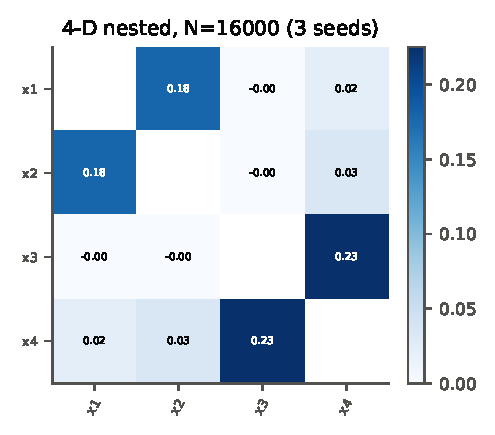
\includegraphics[width=0.92\linewidth]{figs/synergy.pdf}
\caption{Synergy deficits (\cref{def:operators}): validation MSE of the funnel pair forest
minus that of one tree over the pair, divided by $\Var(Y)$.  The 4-D target $\exp\bigl(\tfrac12(\sin\pi(x_1^2+x_2^2)+\sin\pi(x_3^2+x_4^2))\bigr)$; the
two blocks stand out and the cross-block deficits are near zero.}
\label{fig:synergy}
\end{figure}

\paragraph{Synergy.}
\Cref{fig:synergy} estimates the synergy deficit of every pair of coordinates, the
quantity step~2 of \cref{proc:induction} thresholds.  On the 4-D target the within-block
deficits are $0.18$ and $0.23$ of $\Var(Y)$ and the cross-block deficits are within
$0.04$ of zero, so the threshold recovers the blocks $\{x_1,x_2\}$ and $\{x_3,x_4\}$.  The deficit vanishes
whenever both activations are injective functions of their cues, whatever the
interaction (\cref{def:operators}), so a positive deficit marks an interaction that the
activations lose, not every interaction.

\begin{table}[t]
\centering\small
\resizebox{\linewidth}{!}{\begin{tabular}{@{}lrlrrrrr@{}}\toprule
target & $N$ & induced groups ($\tau=0.05$) & one tree & balanced & selected & best & seeds\\\midrule
I.12.11 & 4000 & $\{q\} \{E_f\} \{B,v,\theta\}$ & 0.216 & 0.594 & 0.212 & 0.212 & 3\\
I.13.12 & 4000 & $\{m_1\} \{m_2\} \{r_1\} \{r_2\} \{G\}$ & 0.311 & 0.634 & 0.311 & 0.311 & 3\\
I.29.16 & 4000 & $\{x_1\} \{x_2\} \{\theta_1,\theta_2\}$ & 0.217 & 0.853 & 0.217 & 0.217 & 3\\
I.37.4 & 4000 & $\{I_1\} \{I_2\} \{\delta\}$ & 0.106 & 0.299 & 0.106 & 0.106 & 3\\
I.50.26 & 4000 & $\{x_1\} \{\omega,t\} \{\alpha\}$ & 0.345 & 0.826 & 0.327 & 0.326 & 3\\
I.6.20 & 4000 & $\{\sigma,\theta\}$ & 0.023 & 0.350 & 0.023 & 0.023 & 3\\
I.6.20b & 4000 & $\{\sigma\} \{\theta,\theta_1\}$ & 0.083 & 0.536 & 0.083 & 0.083 & 3\\
I.9.18 & 4000 & $\{m_1\} \{m_2\} \{x_2\} \{x_1\} \{y_2\} \{y_1\} \{z_2\} \{z_1\} \{G\}$ & 0.438 & 0.602 & 0.438 & 0.438 & 3\\
II.6.15a & 4000 & $\{\epsilon,r\} \{p_d\} \{x,y\} \{z\}$ & 0.519 & 0.562 & 0.546 & 0.494 & 3\\
nested4 & 4000 & $\{x_1,x_2\} \{x_3,x_4\}$ & 0.450 & 0.607 & 0.407 & 0.407 & 3\\
nested4 & 16000 & $\{x_1,x_2\} \{x_3,x_4\}$ & 0.300 & 0.626 & 0.294 & 0.294 & 3\\
\bottomrule\end{tabular}}
\caption{Task induction end to end (\cref{proc:induction} and \cref{proc:recipe}, steps 1--4; three seeds, $\kappa=0.25$ for every
candidate).  Groups formed by step~2 at threshold $\tau=0.05$ (most frequent
over seeds, each run estimating its own deficits) and test RMSE$/\mathrm{sd}$ of the
single tree, of the generic balanced forest over the inputs, of the forest selected on
validation data among the single tree, the balanced forest and the induced forests for
$\tau\in\{0.02,0.05,0.1,0.2\}$ with activation or hybrid messages, and of the best
candidate in hindsight.}
\label{tab:induce}
\end{table}

\paragraph{Task induction.}
\Cref{tab:induce} runs \cref{proc:induction} end to end.  The groups it forms are the
interactions that activations lose: in $q(E_f+Bv\sin\theta)$ it merges $B$, $v$ and
$\theta$ and keeps $E_f$ apart, and it also keeps $q$ apart, although $q$ multiplies every
term, because $q$'s activation is injective; in $I.6.20b$ it merges $\theta$ with
$\theta_1$, whose difference the formula uses; in $I.29.16$ it merges the two angles; on
the 4-D target it recovers the two blocks.  The selected forest equals the best candidate,
or is within one percent of it, in every row but one; it beats the single tree on the 4-D target and narrowly on $I.12.11$ and $I.50.26$, and it falls back
on the single tree on the other formulas.
The exception is $II.6.15a$, where the selected forest ($0.546$) is worse than the single
tree ($0.519$), which was among the candidates.  The generic balanced forest is the worst
design on every formula: a forest needs the right graph, and verification at the
composing tree finds one.

\begin{figure}[t]
\centering
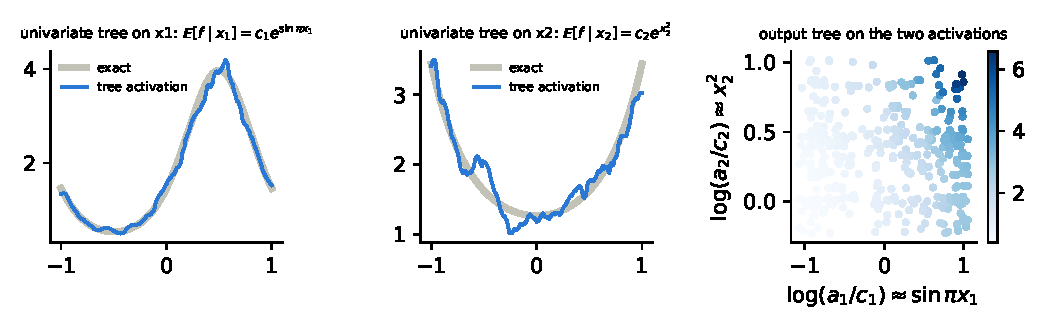
\includegraphics[width=\linewidth]{figs/interpret.pdf}
\caption{What the univariate trees of a funnel forest learn on $\exp(\sin\pi x_1+x_2^2)$
($N=4000$).  Left and centre: each tree's activation against the exact conditional
expectation $\E[f\mid x_i]$.  Right: the output tree's prediction as a function of the
two activations.}
\label{fig:interpret}
\end{figure}

\paragraph{Interpretability.}
Every tree of a forest can be plotted against its inputs.  On
$\exp(\sin\pi x_1+x_2^2)$ the univariate trees learn $c_1e^{\sin\pi x_1}$ and $c_2e^{x_2^2}$
(\cref{fig:interpret}), the inner functions of the target up to the monotone maps
$H_S$ of \cref{prop:suffclass}, without gradients.

\begin{figure}[t]
\centering
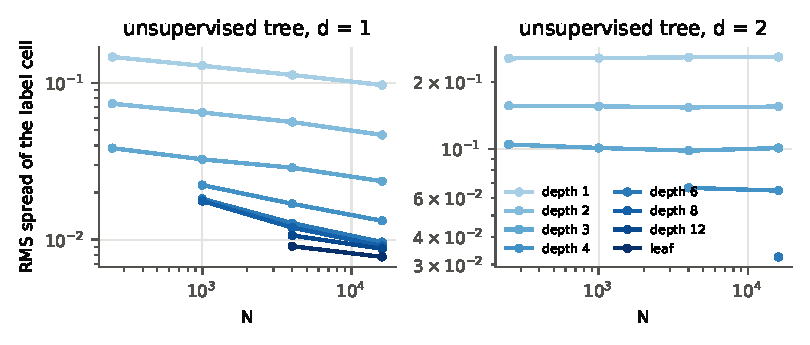
\includegraphics[width=0.8\linewidth]{figs/label_cells.pdf}
\caption{Spread of the cell of a label at fixed depth, for unsupervised trees over
uniform data.}
\label{fig:cells}
\end{figure}

\paragraph{Label cells.}
\Cref{thm:labelcons} needs the cells of the labels to shrink.  In one dimension the cells
of a fixed depth shrink slowly as the tree grows; in two dimensions they do not
(\cref{fig:cells}).  Labels become fine enough only if their depth grows with $N$; the
depths our experiments try are fixed ($2$ to $6$), so the label forests of this section
are outside \cref{thm:labelcons}.  We also tried the cognitively attractive choice of the
\emph{basic level}---the concept of largest expected pointwise mutual information on the
branch, which Cobweb computes: for continuous attributes it lies near the leaves (mean
depth $10$ to $11$), because a concept's information grows as its variance shrinks
towards the variance floor, and its labels did worse than any fixed depth on $xy$.